\documentclass[12pt,a4paper]{article}

\usepackage{amsmath, amssymb, tikz, geometry, tabularx}
\geometry{margin=1in}
\setlength{\parskip}{6pt}

\title{Vector Worksheet}
\author{}
\date{}

\begin{document}
\maketitle
\thispagestyle{empty}

\section*{Vector Representations}

Use the diagram and the partially completed table to fill in the \textbf{three representations} for each vector:
\[
\text{(i)  algebraic variable (usually bold)  \( \mathbf{v}\),\quad }
\text{(ii)  directed path  \( \overrightarrow{AB}\),\quad }
\text{(iii) column vector }
\begin{pmatrix} x \\ y \end{pmatrix}.
\]

For the last columns, create examples of your own

\begin{center}
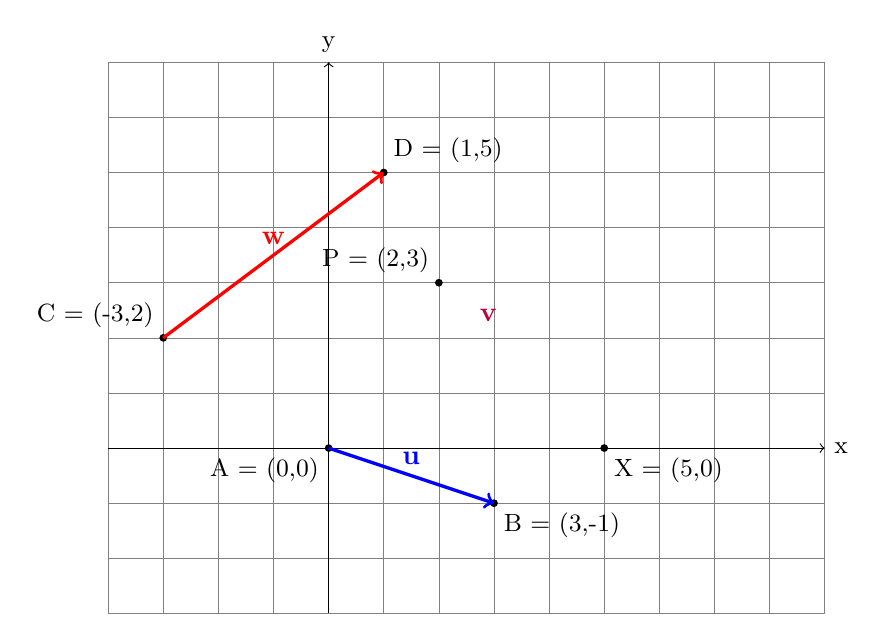
\begin{tikzpicture}[scale=0.7]
  % Grid and axes
  \draw[help lines, step=1] (-4,-3) grid (9,7);
  \draw[->] (-4,0) -- (9,0) node[right]{\small x};
  \draw[->] (0,-3) -- (0,7) node[above]{\small y};

  % u: A(0,0) to B(3,-1) -- complete
  \fill (0,0) circle (2pt) node[below left]{\small A = (0,0)};
  \fill (3,-1) circle (2pt) node[below right]{\small B = (3,-1)};
  \draw[->, very thick, blue] (0,0) -- (3,-1) node[midway, above]{\(\mathbf{u}\)};

  % v: starts at P(2,4) -- end not shown (students add Q)
  \fill (2,3) circle (2pt) node[above left]{\small P = (2,3)};
  \node[purple] at (2.9,2.4) {\(\mathbf{v}\)};
  % (Deliberately no arrow drawn; students draw to Q.)

  % w: C(-3,2) to D(1,5) -- complete
  \fill (-3,2) circle (2pt) node[above left]{\small C = (-3,2)};
  \fill (1,5) circle (2pt) node[above right]{\small D = (1,5)};
  \draw[->, very thick, red] (-3,2) -- (1,5) node[midway, above]{\(\mathbf{w}\)};

  % t: student’s own vector starts at X(5,0) -- end not shown
  \fill (5,0) circle (2pt) node[below right]{\small X = (5,0)};
  % (Students choose and draw end point Y for \mathbf{t}.)
\end{tikzpicture}
\end{center}

\vspace{0.5cm}

\begin{center}
\small
\begin{tabularx}{\textwidth}{|>{\raggedright\arraybackslash}p{2cm}|>{\centering\arraybackslash}p{2cm}|>{\centering\arraybackslash}p{2cm}|>{\centering\arraybackslash}p{2.2cm}|>{\centering\arraybackslash}p{2.2cm}|}
\hline
& \textbf{\(\mathbf{u}\)} & \textbf{\(\mathbf{v}\)} & \textbf{\underline{\hspace{1.6cm}} } & \textbf{\underline{\hspace{1.6cm}} } \\
\hline

\textbf{Points } 
&
\(\;A = (0,0) \newline B = (3,-1) \)
&
\(\;P(2,3) \newline Q = (\underline{\hspace{0.8cm}})\)
&
\(\;C = (-3,2) \newline D = (1,5)\)
&
\(\;X = (5,0) \newline \underline{\hspace{0.5cm}} = (\underline{\hspace{0.8cm}})\)
\\
\hline

\textbf{Directed \newline path}
&
\( \newline \overrightarrow{AB} \)
&
\(\newline \overrightarrow{\boxed{\phantom{aaa}}} \)
&
\(\newline \overrightarrow{\boxed{\phantom{aaa}}} \)
&
\(\newline \overrightarrow{\boxed{\phantom{aaa}}} \)
\\
\hline



\textbf{Column \newline vector}
&
\(\begin{pmatrix} 3 \\ -1 \end{pmatrix}\)
&
\(\begin{pmatrix} 5 \\ 3 \end{pmatrix}\)
&
\(\begin{pmatrix}
\underline{\hspace{0.5cm}} \\[4pt]
\underline{\hspace{0.5cm}}
\end{pmatrix}\)
&
\(\begin{pmatrix}
\underline{\hspace{0.5cm}} \\[4pt]
\underline{\hspace{0.5cm}}
\end{pmatrix}\)
\\
\hline
\end{tabularx}
\end{center}

\vspace{0.5cm}

\section*{Adding vectors}

Use the vectors provided to find a route through the track, that crosses the finish line, you may not leave the grey track, but can touch the sides.

---

Vectors:

\[
\begin{aligned}
\mathbf{a} &= \begin{pmatrix} 3 \\ 2 \end{pmatrix}, &
\mathbf{b} &= \begin{pmatrix} -3 \\ 2 \end{pmatrix}, &
\mathbf{c} &= \begin{pmatrix} 2 \\ -4 \end{pmatrix}, &
\mathbf{d} &= \begin{pmatrix} -2 \\ -3 \end{pmatrix}, \\[6pt]
\mathbf{e} &= \begin{pmatrix} 2 \\ -1 \end{pmatrix}, &
\mathbf{f} &= \begin{pmatrix} -4 \\ -1 \end{pmatrix}, &
\mathbf{g} &= \begin{pmatrix} 1 \\ 3 \end{pmatrix}, &
\mathbf{h} &= \begin{pmatrix} -1 \\ 4 \end{pmatrix}
\end{aligned}
\]

\begin{center}
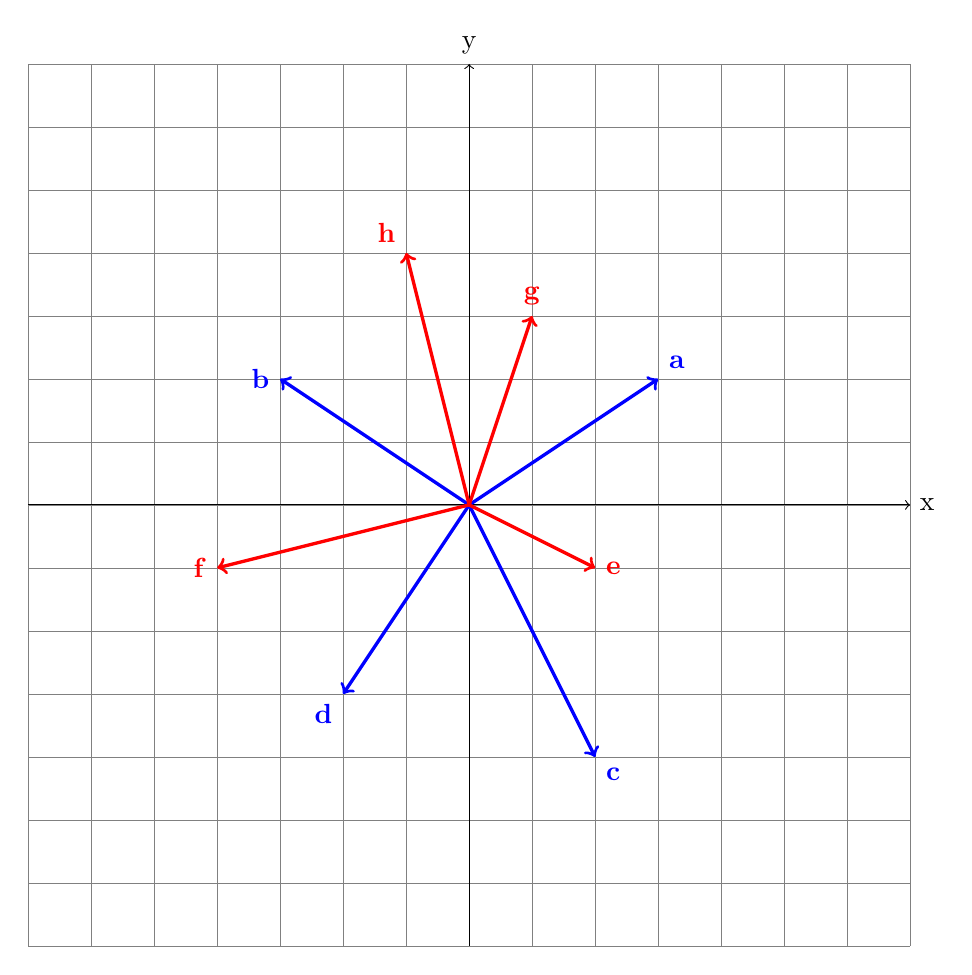
\begin{tikzpicture}[scale=0.8]

    % Grid + axes
    \draw[help lines, step=1] (-7,-7) grid (7,7);
    \draw[->] (-7,0) -- (7,0) node[right] {x};
    \draw[->] (0,-7) -- (0,7) node[above] {y};

    \tikzset{vec/.style={->, very thick}}

    % New varied vectors
    \draw[vec,blue] (0,0) -- (3,2)   node[midway, below right]{} node[above right]{\(\mathbf{a}\)};
    \draw[vec,blue] (0,0) -- (-3,2)  node[midway, above left]{} node[left]{\(\mathbf{b}\)};
    \draw[vec,blue] (0,0) -- (2,-4)  node[midway, right]{} node[below right]{\(\mathbf{c}\)};
    \draw[vec,blue] (0,0) -- (-2,-3) node[midway, left]{} node[below left]{\(\mathbf{d}\)};

    \draw[vec,red]  (0,0) -- (2,-1)  node[midway, above right]{} node[right]{\(\mathbf{e}\)};
    \draw[vec,red]  (0,0) -- (-4,-1) node[midway, above left]{} node[left]{\(\mathbf{f}\)};
    \draw[vec,red]  (0,0) -- (1,3)   node[midway, right]{} node[above]{\(\mathbf{g}\)};
    \draw[vec,red]  (0,0) -- (-1,4)  node[midway, left]{} node[above left]{\(\mathbf{h}\)};

\end{tikzpicture}
\end{center}

---

\begin{center}
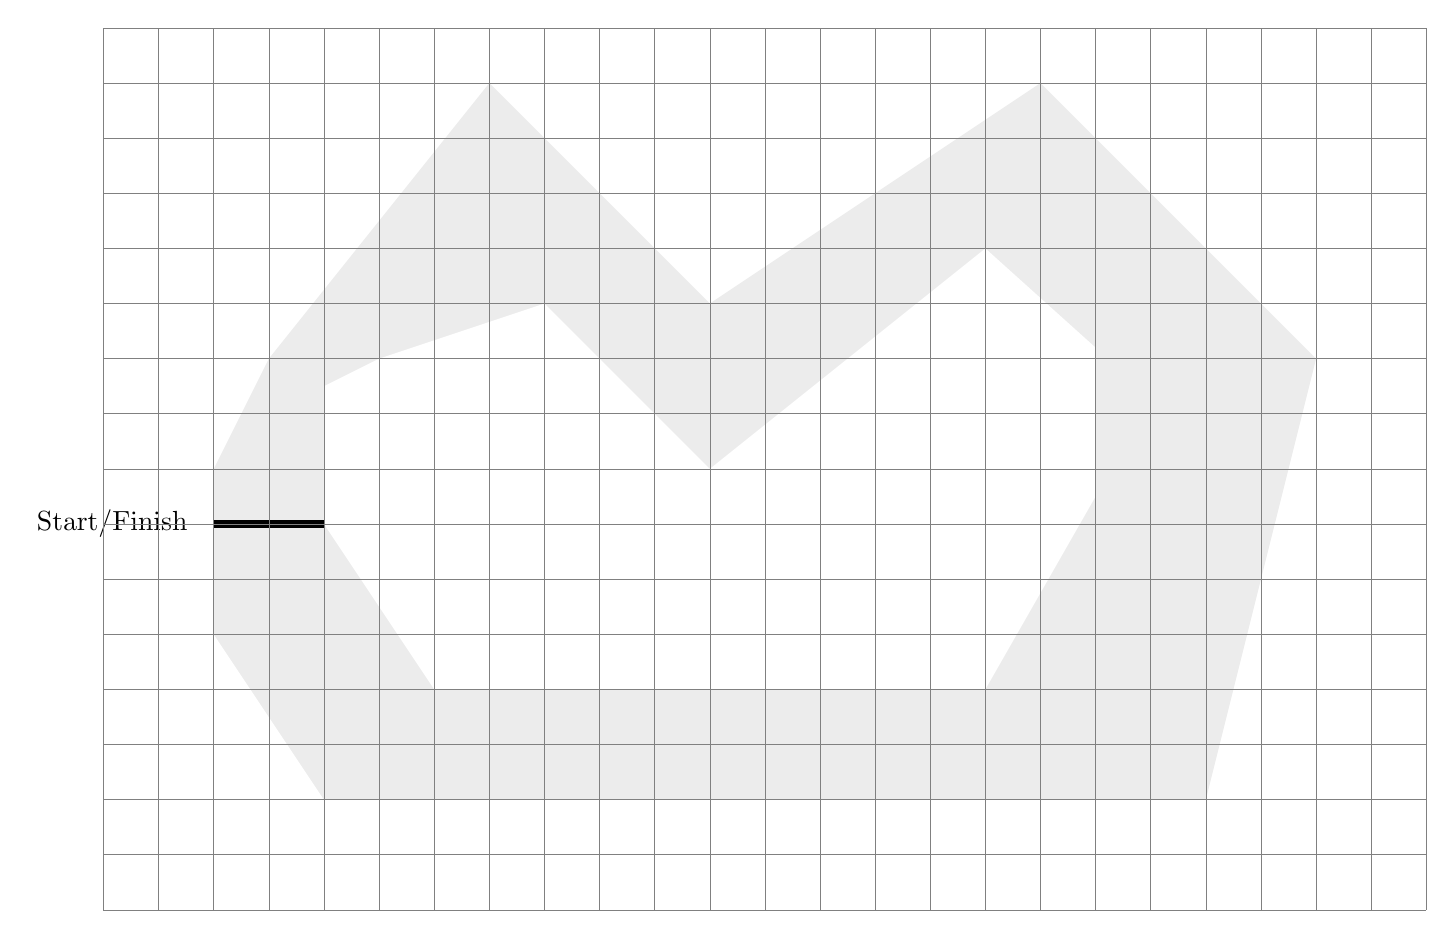
\begin{tikzpicture}[scale=0.7]
    % Grid underneath everything

    % --- Inner boundary (moved inward -> wider track) ---
    % Shifted inward by approx 2 units everywhere
    \draw[line width=3pt, rounded corners=26pt]
        (-8,-1)
        -- (-6,-4)
        -- (3,-4)
        -- (3,-2.5)
        -- (6,2.2)
        -- (3.2,4)
        -- (-1,2)
        -- (-4,4)
        -- (-7,2)
        -- (-8,1.5)
        -- cycle;

    % --- Fill the track band lightly, but keep grid visible ---
    \begin{scope}
        % Clip to the outer boundary
        \clip (-10,-3)
            -- (-8,-6)
            -- (8,-6)
            -- (9,-2)
            -- (10,2)
            -- (5,7)
            -- (-1,3)
            -- (-5,7)
            -- (-9,2)
            -- (-10,0)
            -- cycle;

        % Fill track band
        \fill[gray!15] (-12,-8) rectangle (12,8);

        % Punch out widened inner track
        \fill[white]
            (-8,-1)
            -- (-6,-4)
            -- (4,-4)
            -- (6,-0.5)
            -- (6,2.2)
            -- (4,4)
            -- (-1,0)
            -- (-4,3)
            -- (-7,2)
            -- (-8,1.5)
            -- cycle;
    \end{scope}
    % Start/Finish line
    \draw[line width=3pt] (-10,-1) -- (-8,-1);
    \node[anchor=east] at (-10.3,-1) {Start/Finish};

    \draw[help lines, step=1] (-12,-8) grid (12,8);

\end{tikzpicture}
\end{center}

\begin{center}
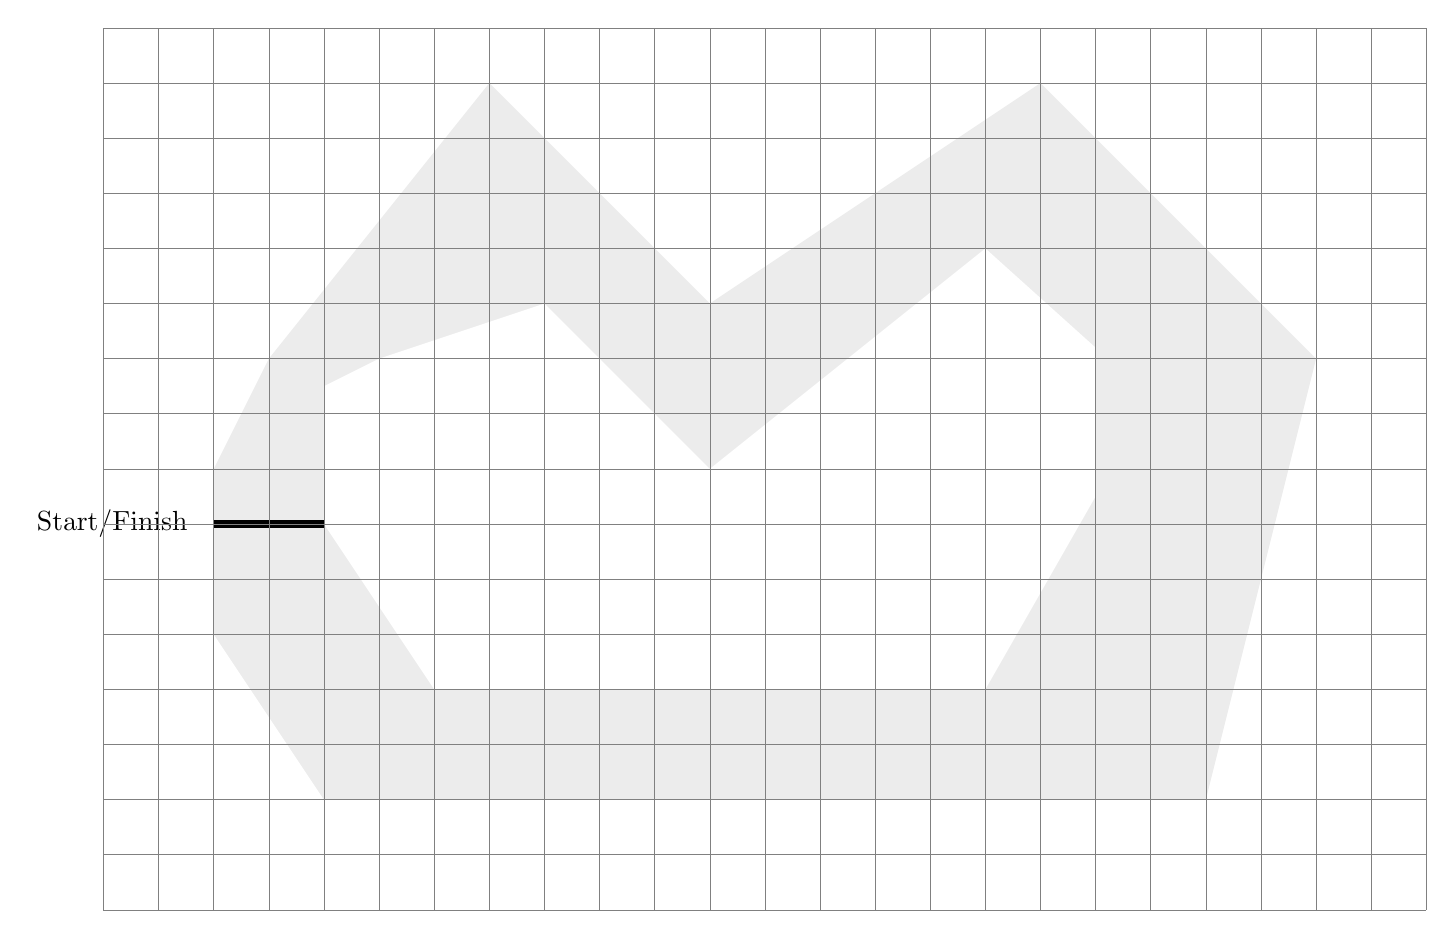
\begin{tikzpicture}[scale=0.7]
    % Grid underneath everything

    % --- Inner boundary (moved inward -> wider track) ---
    % Shifted inward by approx 2 units everywhere
    \draw[line width=3pt, rounded corners=26pt]
        (-8,-1)
        -- (-6,-4)
        -- (3,-4)
        -- (3,-2.5)
        -- (6,2.2)
        -- (3.2,4)
        -- (-1,2)
        -- (-4,4)
        -- (-7,2)
        -- (-8,1.5)
        -- cycle;

    % --- Fill the track band lightly, but keep grid visible ---
    \begin{scope}
        % Clip to the outer boundary
        \clip (-10,-3)
            -- (-8,-6)
            -- (8,-6)
            -- (9,-2)
            -- (10,2)
            -- (5,7)
            -- (-1,3)
            -- (-5,7)
            -- (-9,2)
            -- (-10,0)
            -- cycle;

        % Fill track band
        \fill[gray!15] (-12,-8) rectangle (12,8);

        % Punch out widened inner track
        \fill[white]
            (-8,-1)
            -- (-6,-4)
            -- (4,-4)
            -- (6,-0.5)
            -- (6,2.2)
            -- (4,4)
            -- (-1,0)
            -- (-4,3)
            -- (-7,2)
            -- (-8,1.5)
            -- cycle;
    \end{scope}
    % Start/Finish line
    \draw[line width=3pt] (-10,-1) -- (-8,-1);
    \node[anchor=east] at (-10.3,-1) {Start/Finish};

    \draw[help lines, step=1] (-12,-8) grid (12,8);

\end{tikzpicture}
\end{center}





\newpage{} 

\begin{enumerate}
    \item Write your path in the following form: $g + a + ...$ 
    \vspace{4em}
    \item Collect the like terms in your expression
   \vspace{4em}
   \item Thus evaluate the expression from 1. as a column vector, what do you notice?

\end{enumerate}

\newpage{}

\begin{center}
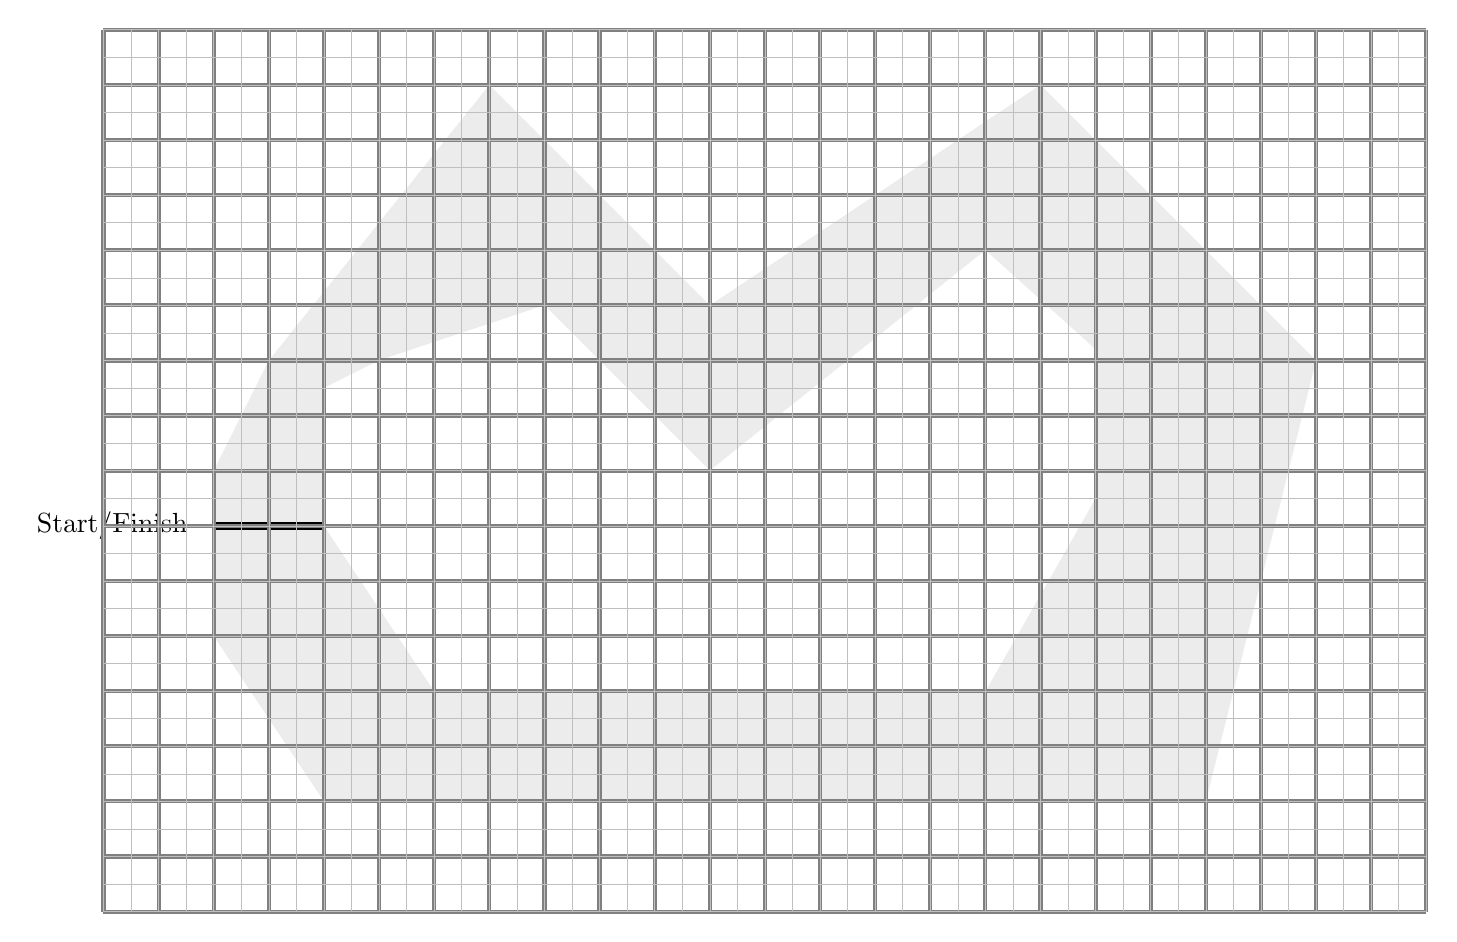
\begin{tikzpicture}[scale=0.7]
    % Grid underneath everything

    % --- Inner boundary (moved inward -> wider track) ---
    % Shifted inward by approx 2 units everywhere
    \draw[line width=3pt, rounded corners=26pt]
        (-8,-1)
        -- (-6,-4)
        -- (3,-4)
        -- (3,-2.5)
        -- (6,2.2)
        -- (3.2,4)
        -- (-1,2)
        -- (-4,4)
        -- (-7,2)
        -- (-8,1.5)
        -- cycle;

    % --- Fill the track band lightly, but keep grid visible ---
    \begin{scope}
        % Clip to the outer boundary
        \clip (-10,-3)
            -- (-8,-6)
            -- (8,-6)
            -- (9,-2)
            -- (10,2)
            -- (5,7)
            -- (-1,3)
            -- (-5,7)
            -- (-9,2)
            -- (-10,0)
            -- cycle;

        % Fill track band
        \fill[gray!15] (-12,-8) rectangle (12,8);

        % Punch out widened inner track
        \fill[white]
            (-8,-1)
            -- (-6,-4)
            -- (4,-4)
            -- (6,-0.5)
            -- (6,2.2)
            -- (4,4)
            -- (-1,0)
            -- (-4,3)
            -- (-7,2)
            -- (-8,1.5)
            -- cycle;
    \end{scope}
    % Start/Finish line
    \draw[line width=3pt] (-10,-1) -- (-8,-1);
    \node[anchor=east] at (-10.3,-1) {Start/Finish};

    \draw[help lines, step=1, line width=1.5pt] (-12,-8) grid (12,8);
    \draw[step=0.5, help lines, color=gray!50] (-12,-8) grid (12,8);


\end{tikzpicture}
\end{center}


\begin{center}
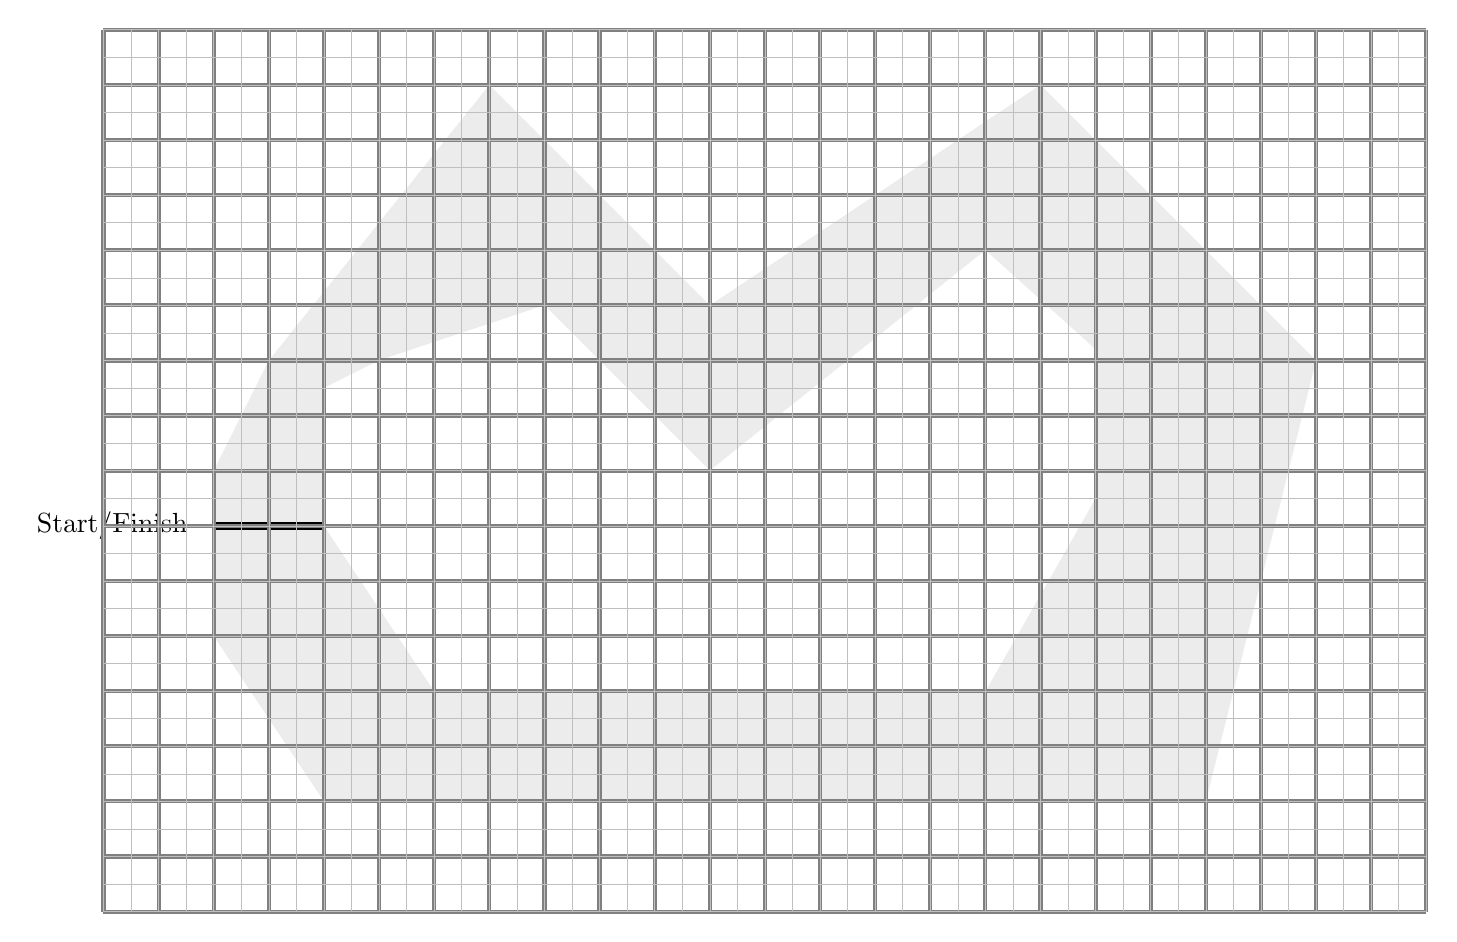
\begin{tikzpicture}[scale=0.7]
    % Grid underneath everything

    % --- Inner boundary (moved inward -> wider track) ---
    % Shifted inward by approx 2 units everywhere
    \draw[line width=3pt, rounded corners=26pt]
        (-8,-1)
        -- (-6,-4)
        -- (3,-4)
        -- (3,-2.5)
        -- (6,2.2)
        -- (3.2,4)
        -- (-1,2)
        -- (-4,4)
        -- (-7,2)
        -- (-8,1.5)
        -- cycle;

    % --- Fill the track band lightly, but keep grid visible ---
    \begin{scope}
        % Clip to the outer boundary
        \clip (-10,-3)
            -- (-8,-6)
            -- (8,-6)
            -- (9,-2)
            -- (10,2)
            -- (5,7)
            -- (-1,3)
            -- (-5,7)
            -- (-9,2)
            -- (-10,0)
            -- cycle;

        % Fill track band
        \fill[gray!15] (-12,-8) rectangle (12,8);

        % Punch out widened inner track
        \fill[white]
            (-8,-1)
            -- (-6,-4)
            -- (4,-4)
            -- (6,-0.5)
            -- (6,2.2)
            -- (4,4)
            -- (-1,0)
            -- (-4,3)
            -- (-7,2)
            -- (-8,1.5)
            -- cycle;
    \end{scope}
    % Start/Finish line
    \draw[line width=3pt] (-10,-1) -- (-8,-1);
    \node[anchor=east] at (-10.3,-1) {Start/Finish};

    \draw[help lines, step=1, line width=1.5pt] (-12,-8) grid (12,8);
    \draw[step=0.5, help lines, color=gray!50] (-12,-8) grid (12,8);

\end{tikzpicture}
\end{center}



\newpage{}


\begin{center}
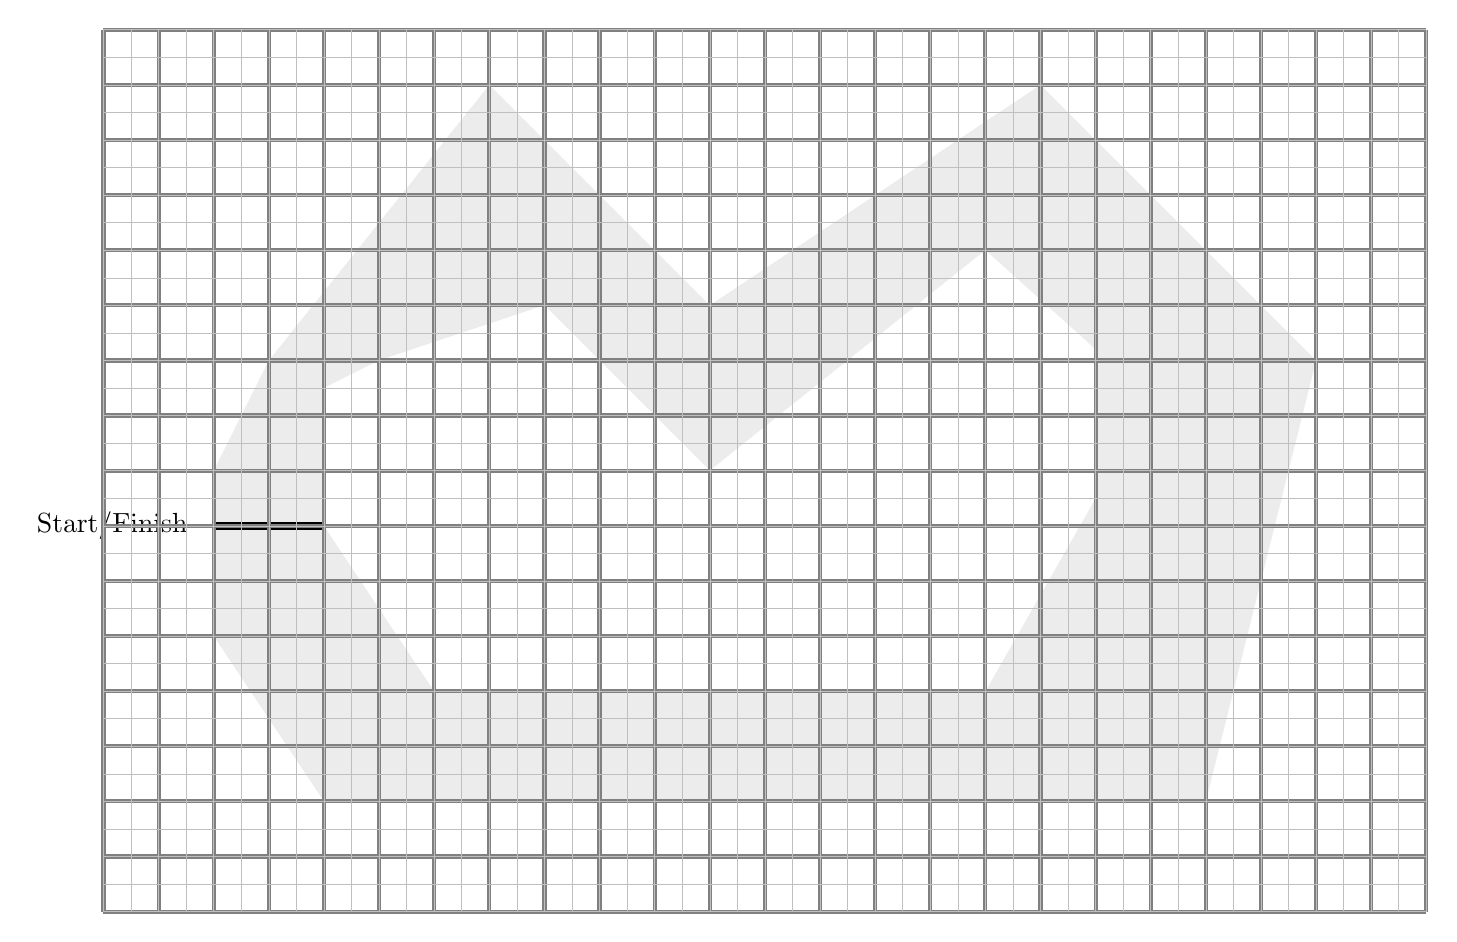
\begin{tikzpicture}[scale=0.7]
    % Grid underneath everything

    % --- Inner boundary (moved inward -> wider track) ---
    % Shifted inward by approx 2 units everywhere
    \draw[line width=3pt, rounded corners=26pt]
        (-8,-1)
        -- (-6,-4)
        -- (3,-4)
        -- (3,-2.5)
        -- (6,2.2)
        -- (3.2,4)
        -- (-1,2)
        -- (-4,4)
        -- (-7,2)
        -- (-8,1.5)
        -- cycle;

    % --- Fill the track band lightly, but keep grid visible ---
    \begin{scope}
        % Clip to the outer boundary
        \clip (-10,-3)
            -- (-8,-6)
            -- (8,-6)
            -- (9,-2)
            -- (10,2)
            -- (5,7)
            -- (-1,3)
            -- (-5,7)
            -- (-9,2)
            -- (-10,0)
            -- cycle;

        % Fill track band
        \fill[gray!15] (-12,-8) rectangle (12,8);

        % Punch out widened inner track
        \fill[white]
            (-8,-1)
            -- (-6,-4)
            -- (4,-4)
            -- (6,-0.5)
            -- (6,2.2)
            -- (4,4)
            -- (-1,0)
            -- (-4,3)
            -- (-7,2)
            -- (-8,1.5)
            -- cycle;
    \end{scope}
    % Start/Finish line
    \draw[line width=3pt] (-10,-1) -- (-8,-1);
    \node[anchor=east] at (-10.3,-1) {Start/Finish};

    \draw[help lines, step=1, line width=1.5pt] (-12,-8) grid (12,8);
    \draw[step=0.5, help lines, color=gray!50] (-12,-8) grid (12,8);

\end{tikzpicture}
\end{center}

\begin{center}
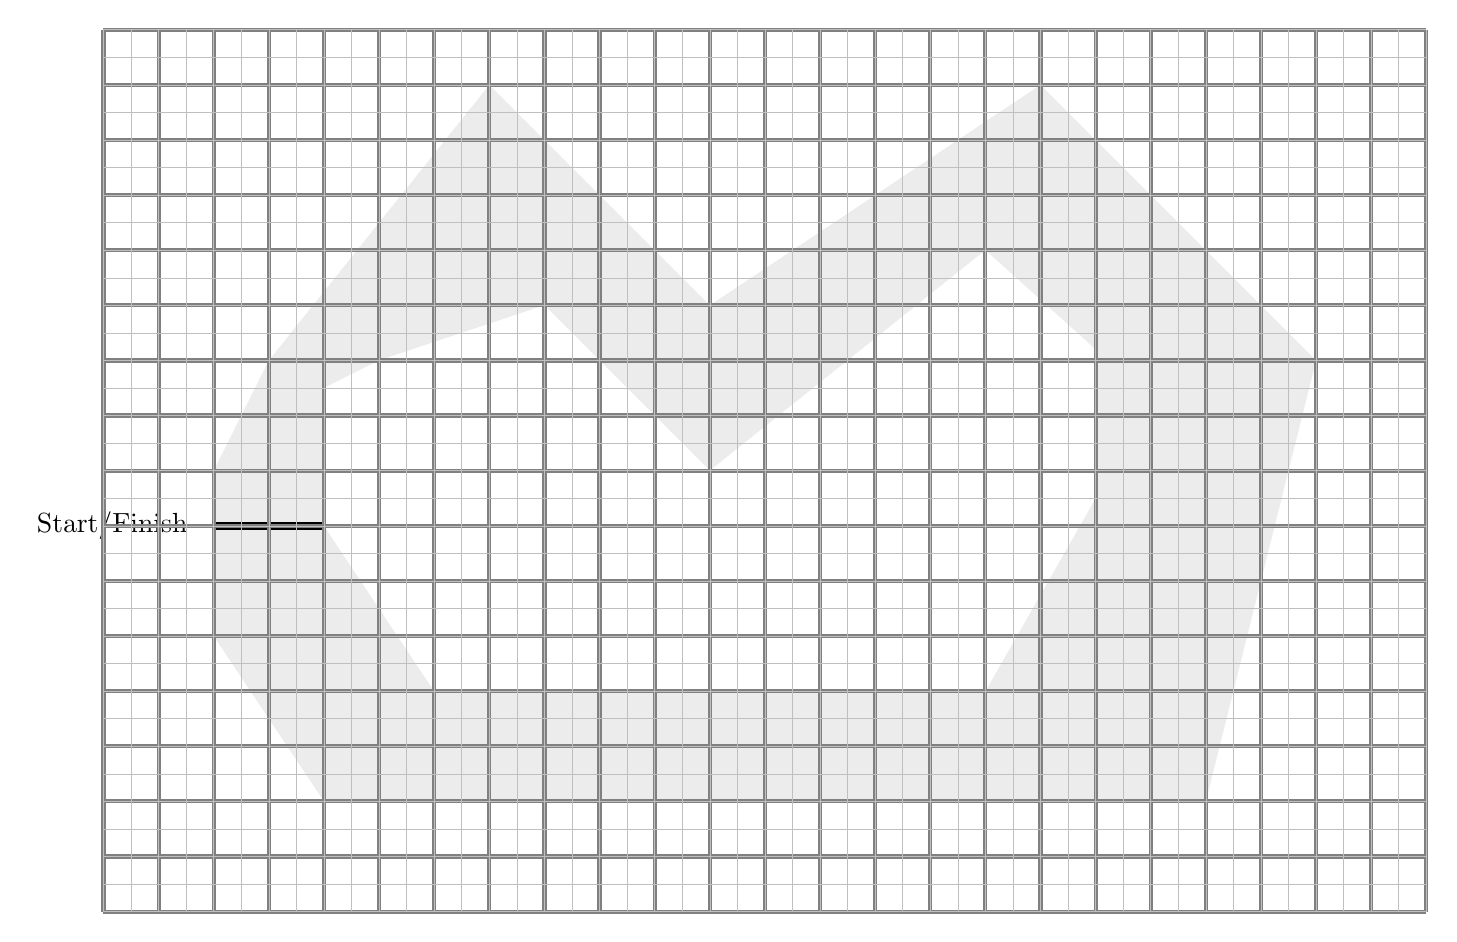
\begin{tikzpicture}[scale=0.7]
    % Grid underneath everything

    % --- Inner boundary (moved inward -> wider track) ---
    % Shifted inward by approx 2 units everywhere
    \draw[line width=3pt, rounded corners=26pt]
        (-8,-1)
        -- (-6,-4)
        -- (3,-4)
        -- (3,-2.5)
        -- (6,2.2)
        -- (3.2,4)
        -- (-1,2)
        -- (-4,4)
        -- (-7,2)
        -- (-8,1.5)
        -- cycle;

    % --- Fill the track band lightly, but keep grid visible ---
    \begin{scope}
        % Clip to the outer boundary
        \clip (-10,-3)
            -- (-8,-6)
            -- (8,-6)
            -- (9,-2)
            -- (10,2)
            -- (5,7)
            -- (-1,3)
            -- (-5,7)
            -- (-9,2)
            -- (-10,0)
            -- cycle;

        % Fill track band
        \fill[gray!15] (-12,-8) rectangle (12,8);

        % Punch out widened inner track
        \fill[white]
            (-8,-1)
            -- (-6,-4)
            -- (4,-4)
            -- (6,-0.5)
            -- (6,2.2)
            -- (4,4)
            -- (-1,0)
            -- (-4,3)
            -- (-7,2)
            -- (-8,1.5)
            -- cycle;
    \end{scope}
    % Start/Finish line
    \draw[line width=3pt] (-10,-1) -- (-8,-1);
    \node[anchor=east] at (-10.3,-1) {Start/Finish};

    \draw[help lines, step=1, line width=1.5pt] (-12,-8) grid (12,8);
    \draw[step=0.5, help lines, color=gray!50] (-12,-8) grid (12,8);

\end{tikzpicture}
\end{center}


\end{document}